\chapter{段差検知システムの検証}
 この章では,構築した段差検知システムについての検証結果を示し,その考察を述べる.

\section{信号処理結果}
 取得したRADARのデータを前章で構築したアルゴリズムに入力し,動作を確認した.図\ref{fig:System_Block_Color}における「5. deffrential」の出力結果,すなわち路面までの距離の微分値の絶対値を図\ref{fig:result_radar}に示す.この値が閾値(今回は0.7)を超えた場合に段差検知とする.段差検知は図中の赤線で示した箇所で発生しており,0.405秒と0.610秒で段差を検出していた.
\begin{figure}[H]
    \centering
    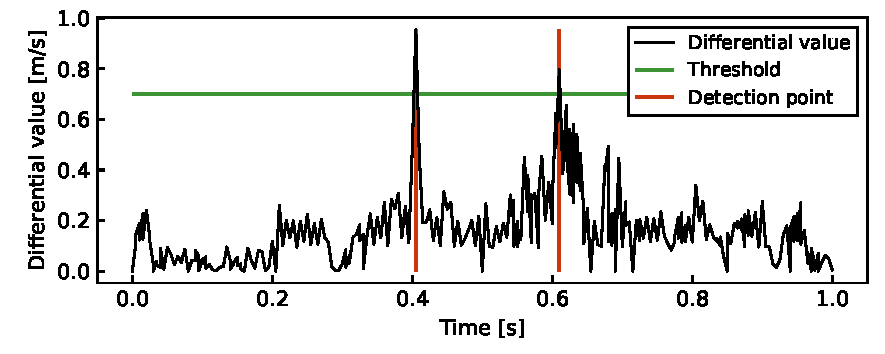
\includegraphics[width=11.5cm]{./fig/result_radar.pdf}
    \caption{路面までの距離の微分値の絶対値}
    \label{fig:result_radar}
\end{figure}

\section{考察}
 

\begin{figure}[H]
    \centering
    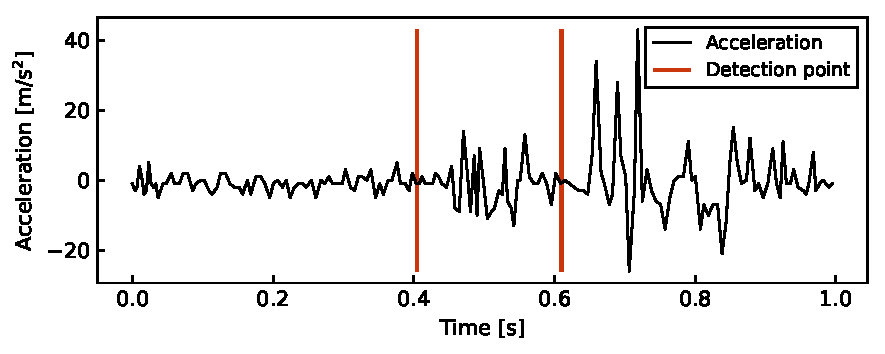
\includegraphics[width=11.5cm]{./fig/result_acc.pdf}
    \caption{車体に加わった上下方向の加速度}
    \label{fig:result_acc}
\end{figure}
